%% Appendix. For the GECCO submission this part goes into the
%% (anonymised) supplementary material; it is compiled after the
%% references so the main paper stays within 8 pages.
\clearpage
\appendix

\section{Reading the Generator: Details}\label{app:reading}

\paragraph{Probes per layer and position.}
Figure~\ref{fig:probes-all} shows every probe target for the three
models, per layer and position. Three patterns hold across models.
First, the outcome of the child is decodable from the generated code
(black) much better than from the prompt (blue, orange): failure is a
property of what is written, not of what is asked. Second, parent
fitness is decodable from the prompt in all positions, as it should be,
since the prompt contains the parent and its score. Third, whether the
child improves on its parent is hardly decodable, and the probe adds
nothing to metadata and text in any model: nothing in the state
predicts progress.
Table~\ref{tab:incremental} gives the incremental value of the probe
over the baselines. For the crash, the probe adds to metadata and text
in all three models; for over-budget children it adds only in Qwen3-8B,
because the parent's outcome already predicts most of it; for child
fitness, it adds only in Gemma-3-12B, whose text baselines are weak.

\begin{figure*}[t]
  \centering
  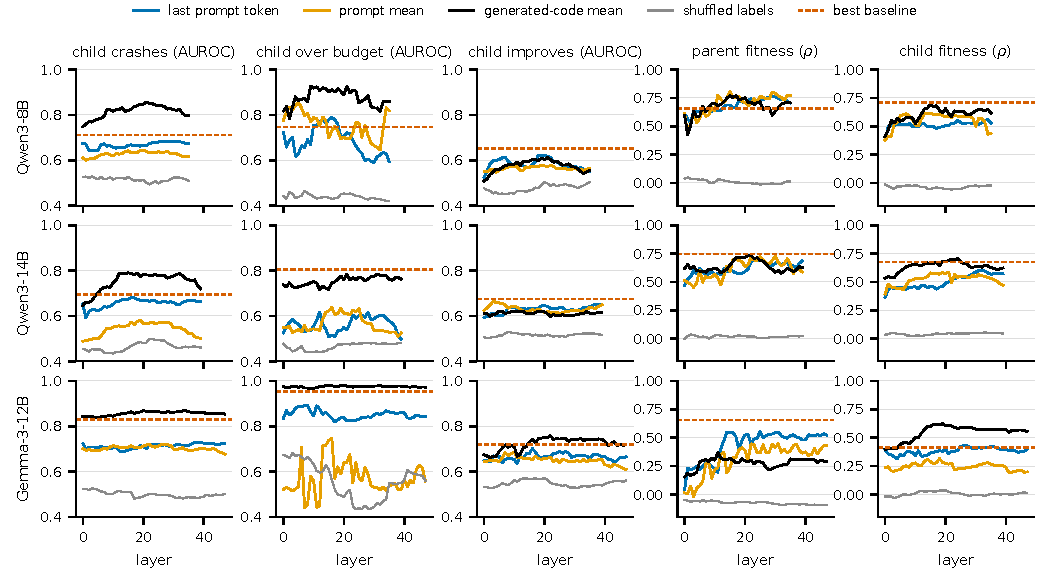
\includegraphics[width=\textwidth]{figures/probes_all}
  \caption{Probe scores per layer for all targets (columns) and models
    (rows), at three positions: last prompt token, mean over the prompt,
    and mean over the generated code. Grey: the generated-code probe on
    shuffled labels. Dashed: the best single baseline (metadata, code
    text or output uncertainty). Child-outcome probes use the generated
    code, which the model writes itself; parent fitness is in the prompt.}
  \Description{A grid of 15 line plots. The generated-code probe is
    highest for crashes and over-budget children in all three models;
    no probe exceeds the baseline for child improvement.}
  \label{fig:probes-all}
\end{figure*}

%% generated by figures/make_appendix.py; do not edit
\begin{table*}[t]
  \caption{Incremental value of the code-state probe (mean over the generated code, best layer chosen inside the folds) over search metadata (M) and code text with output uncertainty (T); nested leave-one-run-out, AUROC or Spearman $\rho$; $\Delta$ is M+T+P $-$ M+T with a 95\% bootstrap CI.}
  \label{tab:incremental}
  \small
  \setlength{\tabcolsep}{3.5pt}
  \begin{tabular}{llrrrrl}
    \toprule
    Model & Target & M & M+T & P & M+T+P & $\Delta$ [95\% CI]\\
    \midrule
    Qwen3-8B & crash & 0.64 & 0.77 & 0.85 & 0.85 & \textbf{+0.08} [+0.05, +0.11]\\
     & over budget & 0.91 & 0.93 & 0.94 & 0.96 & \textbf{+0.03} [+0.01, +0.08]\\
     & improves & 0.66 & 0.68 & 0.61 & 0.68 & $-$0.00 [$-$0.01, +0.01]\\
     & child fitness ($\rho$) & 0.77 & 0.80 & 0.68 & 0.81 & +0.01 [$-$0.01, +0.03]\\
    \midrule
    Qwen3-14B & crash & 0.60 & 0.70 & 0.76 & 0.76 & \textbf{+0.06} [+0.03, +0.09]\\
     & over budget & 0.85 & 0.90 & 0.84 & 0.91 & +0.01 [$-$0.01, +0.03]\\
     & improves & 0.67 & 0.69 & 0.62 & 0.69 & $-$0.00 [$-$0.01, +0.01]\\
     & child fitness ($\rho$) & 0.71 & 0.76 & 0.68 & 0.78 & +0.01 [$-$0.02, +0.04]\\
    \midrule
    Gemma-3-12B & crash & 0.72 & 0.84 & 0.86 & 0.86 & \textbf{+0.02} [+0.01, +0.03]\\
     & over budget & 0.80 & 0.85 & 0.96 & 0.85 & $-$0.00 [$-$0.07, +0.05]\\
     & improves & 0.74 & 0.77 & 0.69 & 0.76 & $-$0.01 [$-$0.02, +0.01]\\
     & child fitness ($\rho$) & 0.43 & 0.53 & 0.61 & 0.62 & \textbf{+0.09} [+0.06, +0.12]\\
    \bottomrule
  \end{tabular}
\end{table*}


\paragraph{Pre-screen.}
Table~\ref{tab:prescreen-rules} compares threshold rules offline on the
unscreened runs of the pre-registered test. All rules flag about a
quarter of the children and catch about 70\% of the failures, at a cost
of 15--17\% of the working children and 11--14\% of the top decile. The
calibrated rules gain nothing over a fixed threshold, so we kept the
simplest. Table~\ref{tab:prescreen-transfer} shows the transfer of the
frozen probe to the transfer screens of Sec.~\ref{sec:steering}: the
MA-BBOB threshold flags almost every child on Bragg and packing, whose
failure rates are 70\% and 51\%, but ranking by the frozen score is
nearly as good as a probe fit on the problem itself.

%% generated by figures/make_appendix.py; do not edit
\begin{table*}[t]
  \caption{Threshold rules for the pre-screen, applied offline to the 3,600 children of the 36 unscreened (shadow) runs, where every child is evaluated (failure rate 16.5\%). Caught: share of the failures flagged; lost: share of the working children (and of the top decile) that would have been skipped.}
  \label{tab:prescreen-rules}
  \small
  \setlength{\tabcolsep}{3.5pt}
  \begin{tabular}{lrrrrr}
    \toprule
    Rule & flagged & caught & working lost & top 10\% lost & precision\\
    \midrule
    fixed threshold & 25\% & 71\% & 16\% & 11\% & 46\%\\
    per operator & 25\% & 65\% & 17\% & 14\% & 43\%\\
    calibrated risk & 25\% & 71\% & 16\% & 11\% & 47\%\\
    running quantile & 24\% & 70\% & 15\% & 11\% & 47\%\\
    \bottomrule
  \end{tabular}
\end{table*}

%% generated by figures/make_appendix.py; do not edit
\begin{table*}[t]
  \caption{The probe pre-screen against smoke tests, on the 3,600 children of the 36 unscreened runs (16.5\% fail), every child re-evaluated in the original sandbox. Flagged children are not evaluated in full. Cost: time spent on the screen as a share of the time of all full evaluations, with the sandbox started separately for the smoke test (about 2.6\,s of the 2.7\,s per smoke test is start-up; run inside the full evaluation's sandbox it costs little).}
  \label{tab:smoke}
  \small
  \setlength{\tabcolsep}{3.5pt}
  \begin{tabular}{lrrrrr}
    \toprule
    Screen & flagged & caught & working lost & precision & cost\\
    \midrule
    probe, fixed threshold & 25\% & 71\% & 16\% & 46\% & 0\%\\
    smoke test: 1 instance, 100 evals & 14\% & 85\% & 0\% & 100\% & 55\%\\
    smoke test: 1 instance, full budget & 16\% & 97\% & 0\% & 100\% & 62\%\\
    probe, then smoke test (100) & 29\% & 91\% & 16\% & 52\% & 41\%\\
    oracle & 16\% & 100\% & 0\% & 100\% & 0\%\\
    \bottomrule
  \end{tabular}
\end{table*}

%% generated by figures/make_appendix.py; do not edit
\begin{table*}[t]
  \caption{The frozen MA-BBOB failure probe on the transfer screens (no retraining). Refit: a probe trained on the problem itself (cross-validated). The MA-BBOB threshold skips almost everything; skipping the top 21\% by the frozen score is precise.}
  \label{tab:prescreen-transfer}
  \small
  \setlength{\tabcolsep}{3.5pt}
  \begin{tabular}{lrrlrrrr}
    \toprule
    Problem & $n$ & fail & frozen AUROC & refit & length & skipped & prec.@21\%\\
    \midrule
    Bragg & 408 & 70\% & 0.77 (0.72--0.82) & 0.84 & 0.55 & 100\% & 92\%\\
    packing & 384 & 51\% & 0.72 (0.67--0.77) & 0.73 & 0.57 & 95\% & 79\%\\
    MA-BBOB corpus (reference) & 4712 & 19\% & 0.82 (0.81--0.84) & 0.88 & -- & 52\% & 53\%\\
    \bottomrule
  \end{tabular}
\end{table*}


\paragraph{Counterfactual prompts.}
Table~\ref{tab:counterfactual} lists every variant. Only changes to the
error trace of a crashed parent change the outcome; changes to the
score, the feedback or a budget message do not. Steering along the
probe direction for parent fitness shifts the similarity of the child
to its parent in opposite directions ($-0.03$ up, $+0.03$ down), but
changes neither its failure rate nor its fitness. A random direction at the same norm raises failures, a
reminder that any perturbation at every token has a cost.

%% generated by figures/make_appendix.py; do not edit
\begin{table*}[t]
  \caption{Counterfactual prompts (Qwen3-8B, 96 queries per variant, 4 replicates with common random numbers). Effects are paired differences to the unchanged prompt with 95\% bootstrap CIs; bold: CI excludes 0. Similarity: change in code similarity of child to parent (smaller = larger rewrite).}
  \label{tab:counterfactual}
  \small
  \setlength{\tabcolsep}{3.5pt}
  \begin{tabular}{lrllr}
    \toprule
    Variant & fail (full) & $\Delta$ fail & $\Delta$ score & $\Delta$ sim.\\
    \midrule
    crashed parent: error trace deleted & 0.43 & \textbf{+0.22} [+0.14, +0.33] & \textbf{$-$0.044} [$-$0.080, $-$0.019] & $-$0.06\\
    crashed parent: generic error message & 0.43 & \textbf{+0.16} [+0.09, +0.25] & \textbf{$-$0.025} [$-$0.047, $-$0.004] & $-$0.03\\
    scored parent: feedback deleted & 0.13 & +0.02 [$-$0.04, +0.07] & +0.003 [$-$0.019, +0.023] & +0.00\\
    scored parent: score set to 0.01 & 0.13 & +0.01 [$-$0.02, +0.05] & $-$0.003 [$-$0.017, +0.015] & $-$0.02\\
    scored parent: score set to 0.90 & 0.13 & +0.02 [$-$0.03, +0.08] & $-$0.012 [$-$0.035, +0.012] & $-$0.00\\
    scored parent: budget message added & 0.12 & +0.02 [$-$0.02, +0.05] & +0.013 [$-$0.007, +0.038] & +0.01\\
    scored parent: steer fitness up & 0.13 & +0.04 [$-$0.01, +0.09] & $-$0.008 [$-$0.027, +0.014] & $-$0.03\\
    scored parent: steer fitness down & 0.13 & $-$0.02 [$-$0.06, +0.01] & +0.021 [$-$0.010, +0.057] & +0.03\\
    scored parent: random direction & 0.13 & \textbf{+0.05} [+0.01, +0.10] & $-$0.014 [$-$0.032, +0.003] & +0.00\\
    \bottomrule
  \end{tabular}
\end{table*}


Table~\ref{tab:cf-models} repeats the main variants in Qwen3-14B and
Gemma-3-12B. The score is ignored in all three. The error trace matters
for both Qwen models. Gemma's failure rate is high whatever the prompt
(72\% after a crashed parent), and the trace does not lower it.

%% generated by figures/make_appendix.py; do not edit
\begin{table*}[t]
  \caption{Counterfactual prompts in three models: change in the child's failure rate (95\% bootstrap CI; bold: excludes 0). Upper rows: parents that crashed; lower rows: working parents. Unchanged-prompt failure rates (crashed/working parent): Qwen3-8B 0.43/0.12, Qwen3-14B 0.52/0.12, Gemma-3-12B 0.72/0.36.}
  \label{tab:cf-models}
  \small
  \setlength{\tabcolsep}{3.5pt}
  \begin{tabular}{llll}
    \toprule
    Variant & Qwen3-8B & Qwen3-14B & Gemma-3-12B\\
    \midrule
    error trace deleted & \textbf{+0.22} [+0.14, +0.33] & \textbf{+0.24} [+0.11, +0.37] & +0.01 [$-$0.08, +0.12]\\
    generic error message & \textbf{+0.16} [+0.09, +0.25] & \textbf{+0.18} [+0.06, +0.31] & +0.02 [$-$0.04, +0.09]\\
    feedback deleted & +0.02 [$-$0.04, +0.07] & $-$0.01 [$-$0.05, +0.03] & +0.01 [$-$0.05, +0.09]\\
    score set to 0.01 & +0.01 [$-$0.02, +0.05] & $-$0.03 [$-$0.07, +0.02] & \textbf{+0.08} [+0.01, +0.14]\\
    score set to 0.90 & +0.02 [$-$0.03, +0.08] & $-$0.00 [$-$0.05, +0.04] & +0.04 [$-$0.02, +0.10]\\
    \bottomrule
  \end{tabular}
\end{table*}


\section{Concept Features}\label{app:concepts}

Table~\ref{tab:keyword} shows, per concept, the SAE feature that best
survives masking the lines that contain the concept's keywords. Most
features drop sharply under line masking, which shows that they read
the keywords themselves (elitism, restart, step-size adaptation). The
features for surrogate, covariance, gradient, population, particle
swarm, adaptive parameters and local search stay well above what the
other concepts and the code length predict. The crossover and DE
features also survive masking, but the other concepts predict DE
almost as well (0.95): they read the DE family as a whole.

%% generated by figures/make_appendix.py; do not edit
\begin{table*}[t]
  \caption{Concept features (Qwen3-8B, top-5 SAE features per concept and layer on the discovery half; shown: the one that best survives line masking; validation AUROC). Masking removes the concept's keyword tokens or their whole lines from the per-algorithm maximum. Baselines: the other concepts' labels plus code length, and code length alone. Bold: the feature detects the concept without its lines (AUROC $\ge0.85$ and at least 0.05 above the label baseline).}
  \label{tab:keyword}
  \small
  \setlength{\tabcolsep}{3.5pt}
  \begin{tabular}{llrrrrr}
    \toprule
    Concept & layer/feat. & none & keyword & line & labels & length\\
    \midrule
    surrogate & L27/62130 & 1.00 & 1.00 & \textbf{1.00} & 0.89 & 0.68\\
    differential evolution & L15/30546 & 0.97 & 0.97 & 0.97 & 0.95 & 0.65\\
    crossover & L15/30546 & 0.98 & 0.97 & 0.97 & 0.96 & 0.67\\
    covariance & L15/5776 & 0.99 & 0.97 & \textbf{0.96} & 0.63 & 0.67\\
    gradient & L15/6720 & 0.96 & 0.96 & \textbf{0.94} & 0.70 & 0.55\\
    population & L9/22950 & 0.98 & 0.97 & \textbf{0.93} & 0.86 & 0.74\\
    particle swarm & L27/38837 & 0.93 & 0.93 & \textbf{0.92} & 0.60 & 0.51\\
    adaptive parameters & L15/14313 & 0.90 & 0.90 & \textbf{0.88} & 0.77 & 0.78\\
    local search & L27/26058 & 0.92 & 0.88 & \textbf{0.88} & 0.78 & 0.74\\
    restart & L27/44846 & 0.99 & 0.83 & 0.81 & 0.74 & 0.63\\
    elitism & L27/46445 & 1.00 & 0.88 & 0.76 & 0.74 & 0.66\\
    step size adaptation & L9/3169 & 0.75 & 0.75 & 0.73 & 0.65 & 0.50\\
    \bottomrule
  \end{tabular}
\end{table*}


\section{Steering: Screens and Transfer}\label{app:steering}

\paragraph{Contrastive concept levers.}
Table~\ref{tab:levers} lists the ten contrastive directions for rare
concepts. Four insert their concept at one of the two doses; the others
change failures but not the concept. Even the working levers raise
failures, and at a dose of 0.5 most directions raise the failure rate
by 0.25 or more.

%% generated by figures/make_appendix.py; do not edit
\begin{table*}[t]
  \caption{Contrastive concept directions (layer 15, mean difference of algorithms with and without the concept, 16 prompts per dose): change in the rate of the concept in the generated code (95\% bootstrap CI) and in the failure rate, at doses 0.3 and 0.5 of the residual norm.}
  \label{tab:levers}
  \small
  \setlength{\tabcolsep}{3.5pt}
  \begin{tabular}{lllll}
    \toprule
     & \multicolumn{2}{c}{dose 0.3} & \multicolumn{2}{c}{dose 0.5}\\ Direction & $\Delta$ concept & $\Delta$ fail & $\Delta$ concept & $\Delta$ fail\\
    \midrule
    archive & +0.00 [+0.00, +0.00] & +0.25 & +0.06 [+0.00, +0.19] & +0.62\\
    covariance & \textbf{+0.31} [+0.12, +0.56] & +0.19 & \textbf{+0.38} [+0.12, +0.62] & +0.25\\
    levy flight & +0.00 [+0.00, +0.00] & +0.25 & +0.00 [+0.00, +0.00] & +0.38\\
    local search & \textbf{+0.31} [+0.12, +0.56] & +0.19 & +0.19 [+0.00, +0.38] & +0.56\\
    opposition & +0.00 [+0.00, +0.00] & +0.06 & +0.00 [+0.00, +0.00] & +0.56\\
    quasi random init & +0.00 [+0.00, +0.00] & +0.06 & +0.00 [+0.00, +0.00] & +0.06\\
    restart & +0.19 [+0.00, +0.38] & +0.38 & +0.19 [+0.00, +0.38] & +0.38\\
    simulated annealing & +0.25 [+0.00, +0.50] & +0.12 & \textbf{+0.38} [+0.12, +0.62] & +0.31\\
    surrogate & +0.12 [+0.00, +0.31] & +0.31 & \textbf{+0.44} [+0.19, +0.69] & +0.56\\
    tournament selection & +0.00 [+0.00, +0.00] & +0.12 & +0.00 [+0.00, +0.00] & +0.44\\
    \bottomrule
  \end{tabular}
  \\[2pt]\raggedright\footnotesize Unsteered failure rate 0.12; random direction at the same norm: $\Delta$ fail $-$0.06 (0.3), +0.25 (0.5).
\end{table*}


\paragraph{Transfer screens.}
Table~\ref{tab:transfer} gives the slopes per unit dose of the dial on
each transfer problem. The design-space columns (population, DE, local
search, gradient) move on every problem, while the behaviour columns
(exploration, intensification) move only on Bragg and, weakly, f20.
The quality of the generated code rises with the dose on f2 and f9.

%% generated by figures/make_appendix.py; do not edit
\begin{table*}[t]
  \caption{The MA-BBOB exploration dial applied unchanged to five new problems: slope per unit dose (doses $\pm0.2$, $\pm0.4$ and none; initial and refine prompts pooled; 384--408 samples per problem). Bold: 95\% bootstrap CI excludes 0. Exploration and intensification are measured from the traced evaluations (packing calls no black box); the next four columns are shares of generated code with the concept; score is the problem's fitness of working code.}
  \label{tab:transfer}
  \small
  \setlength{\tabcolsep}{3.5pt}
  \begin{tabular}{lrrrrrrrr}
    \toprule
    Problem & expl.\,\% & intens. & population & DE & local search & gradient & score & fail\\
    \midrule
    Bragg & \textbf{+30} & \textbf{$-$0.45} & \textbf{+0.34} & \textbf{+0.46} & \textbf{$-$0.39} & $-$0.01 & +0.046 & $-$0.03\\
    packing & -- & -- & \textbf{+0.62} & +0.00 & \textbf{$-$0.90} & \textbf{$-$0.12} & +0.030 & \textbf{$-$0.37}\\
    BBOB f20 & +21 & $-$0.11 & \textbf{+0.84} & \textbf{+0.23} & $-$0.02 & \textbf{$-$0.35} & +0.023 & $-$0.16\\
    BBOB f2 & +12 & $-$0.07 & \textbf{+0.66} & \textbf{+0.38} & +0.02 & \textbf{$-$0.41} & \textbf{+0.083} & $-$0.13\\
    BBOB f9 & +4 & +0.02 & \textbf{+0.58} & \textbf{+0.23} & $-$0.03 & $-$0.16 & \textbf{+0.058} & +0.09\\
    \bottomrule
  \end{tabular}
\end{table*}


\section{Steered \llamea: Full Results}\label{app:loop}

\paragraph{MA-BBOB\@.}
Table~\ref{tab:mabbob-b200} gives the paired comparisons at 100 and 200
evaluations, including the area under the best-so-far curve, the number
of seeds on which each arm beats control, and three contrasts between
arms. Table~\ref{tab:mabbob-search} gives the search statistics of the
first 100 evaluations. The exploit dial lowers intensification and
raises the measured exploration of the final algorithms: its code moves
widely without intensifying. The
prompts move exploration in the intended direction, but they write the
fewest families. Table~\ref{tab:mabbob-concepts} shows which concepts
each arm writes: the explore dial and anneal write population-based DE
with crossover; the exploit dial removes DE, crossover and elitism
almost entirely; the exploit prompt writes step-size adaptation and
covariance learning, the words of its instruction.

%% generated by figures/make_appendix.py; do not edit
\begin{table*}[t]
  \caption{Steered \llamea on MA-BBOB: mean best \aocc after 100 and 200 evaluations and area under the best-so-far curve (200), with the paired difference to control and the number of seeds on which the arm beats control. Bold: 95\% bootstrap CI excludes 0. Gain: mean improvement of the best from 100 to 200. Lower block: paired contrasts at 200.}
  \label{tab:mabbob-b200}
  \small
  \setlength{\tabcolsep}{3.5pt}
  \begin{tabular}{lrlllr}
    \toprule
    Arm & seeds & best@100 ($\Delta$, wins) & best@200 ($\Delta$, wins) & area@200 ($\Delta$, wins) & gain\\
    \midrule
    control & 16 & 0.64 & 0.68 & 0.60 & 0.042\\
    adaptive dial & 16 & 0.70 (+0.06, 11) & 0.75 (\textbf{+0.08}, 12) & 0.65 (+0.05, 10) & 0.055\\
    dial explore & 16 & 0.66 (+0.02, 8) & 0.73 (+0.05, 10) & 0.64 (+0.04, 10) & 0.068\\
    dial exploit & 16 & 0.40 (\textbf{$-$0.24}, 3) & 0.49 (\textbf{$-$0.19}, 2) & 0.39 (\textbf{$-$0.21}, 3) & 0.087\\
    dial anneal & 16 & 0.62 ($-$0.01, 6) & 0.70 (+0.02, 6) & 0.60 ($-$0.00, 6) & 0.080\\
    random dir. & 16 & 0.58 ($-$0.06, 6) & 0.66 ($-$0.02, 8) & 0.55 ($-$0.05, 6) & 0.082\\
    prompt explore & 16 & 0.62 ($-$0.02, 7) & 0.69 (+0.01, 7) & 0.58 ($-$0.02, 7) & 0.070\\
    prompt exploit & 16 & 0.59 ($-$0.05, 6) & 0.63 ($-$0.05, 5) & 0.56 ($-$0.04, 6) & 0.042\\
    \midrule
    dial explore $-$ exploit & 16 & & \textbf{+0.24} [+0.16, +0.32] (14) & & \\
    prompt explore $-$ exploit & 16 & & +0.06 [$-$0.00, +0.12] (11) & & \\
    calibrated $-$ adaptive dial & 8 & & $-$0.05 [$-$0.13, +0.03] (3) & & \\
    \bottomrule
  \end{tabular}
\end{table*}

%% generated by figures/make_appendix.py; do not edit
\begin{table*}[t]
  \caption{Search statistics of steered \llamea on MA-BBOB (first 100 evaluations; 16 seeds, anneal and random direction 8): failure rate, number of distinct algorithm families (concept sets) written, concept diversity (mean Jaccard distance), and measured exploration and intensification of the generated algorithms. In brackets: paired difference to control; bold: 95\% CI excludes 0.}
  \label{tab:mabbob-search}
  \small
  \setlength{\tabcolsep}{3.5pt}
  \begin{tabular}{llllll}
    \toprule
    Arm & fail & families & concept div. & expl.\,\% & intens.\\
    \midrule
    control & 0.17 & 26.4 & 0.47 & 23.9 & 0.63\\
    adaptive dial & 0.22 (\textbf{+0.06}) & 32.9 (\textbf{+6.4}) & 0.55 (\textbf{+0.08}) & 29.6 (+5.7) & 0.60 ($-$0.03)\\
    dial explore & 0.17 (+0.01) & 28.1 (+1.7) & 0.42 ($-$0.05) & 32.3 (\textbf{+8.4}) & 0.56 ($-$0.07)\\
    dial exploit & 0.16 ($-$0.01) & 17.9 (\textbf{$-$8.5}) & 0.54 (\textbf{+0.07}) & 35.3 (+11.4) & 0.41 (\textbf{$-$0.22})\\
    dial anneal & 0.14 ($-$0.02) & 27.8 (+2.0) & 0.45 ($-$0.04) & 28.8 (+6.3) & 0.57 ($-$0.09)\\
    random dir. & 0.20 (+0.05) & 23.1 ($-$2.6) & 0.51 (+0.03) & 34.1 (\textbf{+11.6}) & 0.55 (\textbf{$-$0.11})\\
    prompt explore & 0.18 (+0.02) & 14.2 (\textbf{$-$12.2}) & 0.53 (+0.06) & 43.2 (\textbf{+19.3}) & 0.52 (\textbf{$-$0.11})\\
    prompt exploit & 0.13 ($-$0.03) & 19.3 (\textbf{$-$7.1}) & 0.47 (+0.00) & 24.1 (+0.2) & 0.66 (+0.03)\\
    \bottomrule
  \end{tabular}
\end{table*}

%% generated by figures/make_appendix.py; do not edit
\begin{table*}[t]
  \caption{Concepts in the generated algorithms on MA-BBOB: percentage of the algorithms of an arm that contain the concept (pop.: population, DE: differential evolution, cross.: crossover, elit.: elitism, grad.: gradient, step: step-size adaptation, cov.: covariance, LS: local search, SA: simulated annealing, PSO: particle swarm).}
  \label{tab:mabbob-concepts}
  \small
  \setlength{\tabcolsep}{3.5pt}
  \begin{tabular}{lrrrrrrrrrr}
    \toprule
    Arm & pop. & DE & cross. & elit. & grad. & step & cov. & LS & SA & PSO\\
    \midrule
    control & 67 & 37 & 28 & 17 & 66 & 35 & 11 & 4 & 1 & 19\\
    adaptive dial & 82 & 49 & 43 & 27 & 42 & 37 & 19 & 8 & 0 & 11\\
    dial explore & 95 & 75 & 81 & 40 & 40 & 3 & 4 & 19 & 0 & 7\\
    dial exploit & 25 & 1 & 1 & 0 & 58 & 54 & 12 & 2 & 18 & 2\\
    dial anneal & 93 & 63 & 64 & 28 & 52 & 13 & 11 & 29 & 0 & 8\\
    random dir. & 55 & 11 & 11 & 5 & 74 & 48 & 11 & 3 & 0 & 16\\
    prompt explore & 67 & 13 & 15 & 15 & 18 & 25 & 10 & 13 & 0 & 0\\
    prompt exploit & 28 & 6 & 0 & 12 & 44 & 84 & 45 & 15 & 0 & 2\\
    \bottomrule
  \end{tabular}
\end{table*}


\paragraph{Bragg, packing and BBOB\@.}
Table~\ref{tab:bragg-packing} gives the paired results on Bragg and
packing, Table~\ref{tab:bbob-full} those on the three BBOB functions,
and Fig.~\ref{fig:curves-transfer} the best-so-far curves. On BBOB the
picture is consistent across functions: the exploit dial and both
prompts cut the families written by 8 to 18, the exploit side removes
DE, and only on f2, where DE is the winning family, does this cost
fitness.

\begin{figure*}[t]
  \centering
  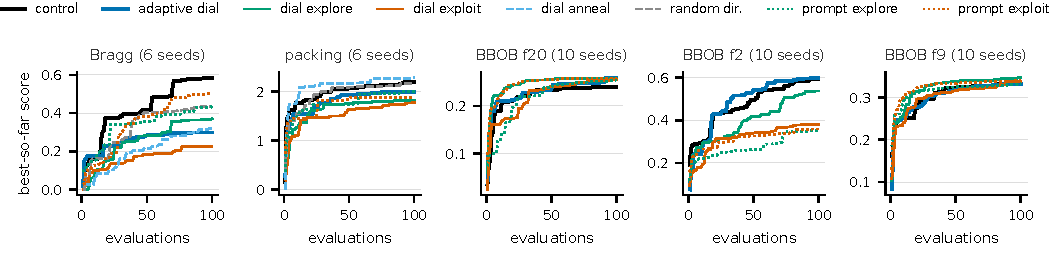
\includegraphics[width=\textwidth]{figures/curves_transfer}
  \caption{Best-so-far score of the steered \llamea arms on the transfer
    problems, mean over seeds (Bragg and BBOB: \aocc; packing: sum of
    radii). Anneal and the random direction were run on Bragg and
    packing only.}
  \Description{Five line plots over 100 evaluations. On Bragg, control
    ends highest at about 0.58 and the dial arms lower; on packing, all
    arms end between 1.8 and 2.3; on f20 and f9 all arms end close
    together; on f2, control and the adaptive dial reach about 0.6, the
    explore dial 0.54 and the exploit and prompt arms below 0.4.}
  \label{fig:curves-transfer}
\end{figure*}

\paragraph{Multiple comparisons.}
Table~\ref{tab:multiplicity} lists every arm-versus-control comparison of
the closed-loop campaigns, with exact sign-flip tests and Holm's
correction. Over all 43 comparisons, none survives. Within a problem,
three do: the exploit dial on MA-BBOB at 100 and at 200 evaluations,
and the explore dial on f9. With 6 seeds (Bragg, packing) no comparison
can survive any correction, so those campaigns can only show large,
consistent effects; their equivalence bounds (0.27--0.82) are wide.
On f20 and f9 the bounds are small (at most 0.05 and 0.02): there,
the arms are practically equivalent.

%% generated by figures/make_appendix.py; do not edit
\begin{table*}[t]
  \caption{Every arm compared with control on the best score of the run, paired by seed: mean difference with 95\% bootstrap CI; equivalence bound (largest $|\Delta|$ inside the 90\% CI, TOST at $\alpha=0.05$); exact two-sided sign-flip $p$; Holm's correction within the problem and over all 43 comparisons. Bold: Holm within the problem $<0.05$. With 6 seeds the smallest attainable $p$ is 1/32.}
  \label{tab:multiplicity}
  \footnotesize
  \setlength{\tabcolsep}{3.5pt}
  \begin{tabular}{lllllrrr}
    \toprule
    Problem & Arm & seeds & $\Delta$ [95\% CI] & equiv. & $p$ & Holm (prob.) & Holm (all)\\
    \midrule
    MA-BBOB @200 & adaptive dial & 16 & +0.076 [+0.020, +0.133] & 0.125 & 0.021 & 0.127 & 0.85\\
     & dial anneal & 16 & +0.024 [$-$0.069, +0.110] & 0.098 & 0.613 & 1.000 & 1.00\\
     & dial exploit & 16 & $-$0.193 [$-$0.302, $-$0.076] & 0.284 & 0.007 & \textbf{0.049} & 0.29\\
     & dial explore & 16 & +0.049 [$-$0.041, +0.133] & 0.121 & 0.305 & 1.000 & 1.00\\
     & prompt exploit & 16 & $-$0.048 [$-$0.120, +0.034] & 0.108 & 0.248 & 1.000 & 1.00\\
     & prompt explore & 16 & +0.008 [$-$0.069, +0.080] & 0.068 & 0.846 & 1.000 & 1.00\\
     & random dir. & 16 & $-$0.019 [$-$0.106, +0.067] & 0.094 & 0.696 & 1.000 & 1.00\\
    \midrule
    MA-BBOB @100 & adaptive dial & 16 & +0.063 [$-$0.015, +0.146] & 0.130 & 0.158 & 0.951 & 1.00\\
     & dial anneal & 16 & $-$0.015 [$-$0.126, +0.102] & 0.111 & 0.812 & 1.000 & 1.00\\
     & dial exploit & 16 & $-$0.238 [$-$0.348, $-$0.121] & 0.330 & 0.002 & \textbf{0.017} & 0.10\\
     & dial explore & 16 & +0.022 [$-$0.077, +0.124] & 0.108 & 0.684 & 1.000 & 1.00\\
     & prompt exploit & 16 & $-$0.049 [$-$0.133, +0.042] & 0.119 & 0.298 & 1.000 & 1.00\\
     & prompt explore & 16 & $-$0.021 [$-$0.125, +0.081] & 0.108 & 0.704 & 1.000 & 1.00\\
     & random dir. & 16 & $-$0.059 [$-$0.161, +0.042] & 0.145 & 0.288 & 1.000 & 1.00\\
    \midrule
    Bragg & adaptive dial & 6 & $-$0.286 [$-$0.496, $-$0.049] & 0.465 & 0.125 & 0.625 & 1.00\\
     & dial anneal & 6 & $-$0.265 [$-$0.434, $-$0.103] & 0.417 & 0.031 & 0.219 & 1.00\\
     & dial exploit & 6 & $-$0.359 [$-$0.561, $-$0.180] & 0.526 & 0.031 & 0.219 & 1.00\\
     & dial explore & 6 & $-$0.213 [$-$0.438, +0.009] & 0.403 & 0.219 & 0.875 & 1.00\\
     & prompt exploit & 6 & $-$0.082 [$-$0.317, +0.144] & 0.275 & 0.531 & 0.938 & 1.00\\
     & prompt explore & 6 & $-$0.149 [$-$0.433, +0.141] & 0.403 & 0.312 & 0.938 & 1.00\\
     & random dir. & 6 & $-$0.152 [$-$0.515, +0.257] & 0.469 & 0.469 & 0.938 & 1.00\\
    \midrule
    packing & adaptive dial & 6 & $-$0.201 [$-$0.602, +0.183] & 0.539 & 0.406 & 1.000 & 1.00\\
     & dial anneal & 6 & +0.091 [$-$0.122, +0.301] & 0.269 & 0.438 & 1.000 & 1.00\\
     & dial exploit & 6 & $-$0.420 [$-$0.620, $-$0.218] & 0.592 & 0.031 & 0.219 & 1.00\\
     & dial explore & 6 & $-$0.368 [$-$0.914, +0.124] & 0.820 & 0.344 & 1.000 & 1.00\\
     & prompt exploit & 6 & $-$0.303 [$-$0.537, $-$0.052] & 0.506 & 0.094 & 0.562 & 1.00\\
     & prompt explore & 6 & $-$0.181 [$-$0.467, +0.085] & 0.423 & 0.375 & 1.000 & 1.00\\
     & random dir. & 6 & $-$0.029 [$-$0.366, +0.298] & 0.319 & 0.875 & 1.000 & 1.00\\
    \midrule
    BBOB f20 & adaptive dial & 10 & +0.019 [$-$0.001, +0.054] & 0.051 & 0.240 & 0.859 & 1.00\\
     & dial exploit & 10 & +0.014 [$-$0.005, +0.047] & 0.045 & 0.607 & 1.000 & 1.00\\
     & dial explore & 10 & +0.018 [$-$0.001, +0.050] & 0.047 & 0.172 & 0.859 & 1.00\\
     & prompt exploit & 10 & +0.018 [$-$0.001, +0.051] & 0.048 & 0.178 & 0.859 & 1.00\\
     & prompt explore & 10 & +0.014 [$-$0.005, +0.048] & 0.046 & 0.768 & 1.000 & 1.00\\
    \midrule
    BBOB f2 & adaptive dial & 10 & +0.005 [$-$0.205, +0.209] & 0.180 & 0.965 & 0.965 & 1.00\\
     & dial exploit & 10 & $-$0.212 [$-$0.396, +0.008] & 0.371 & 0.088 & 0.352 & 1.00\\
     & dial explore & 10 & $-$0.056 [$-$0.168, +0.051] & 0.150 & 0.369 & 0.738 & 1.00\\
     & prompt exploit & 10 & $-$0.234 [$-$0.424, $-$0.004] & 0.399 & 0.076 & 0.352 & 1.00\\
     & prompt explore & 10 & $-$0.241 [$-$0.442, $-$0.009] & 0.413 & 0.070 & 0.352 & 1.00\\
    \midrule
    BBOB f9 & adaptive dial & 10 & $-$0.002 [$-$0.009, +0.003] & 0.008 & 0.596 & 1.000 & 1.00\\
     & dial exploit & 10 & +0.004 [$-$0.004, +0.013] & 0.011 & 0.367 & 1.000 & 1.00\\
     & dial explore & 10 & +0.013 [+0.007, +0.020] & 0.019 & 0.002 & \textbf{0.010} & 0.08\\
     & prompt exploit & 10 & +0.007 [$-$0.002, +0.017] & 0.015 & 0.195 & 0.781 & 1.00\\
     & prompt explore & 10 & +0.000 [$-$0.013, +0.013] & 0.011 & 0.982 & 1.000 & 1.00\\
    \bottomrule
  \end{tabular}
\end{table*}

%% generated by figures/make_appendix.py; do not edit
\begin{table*}[t]
  \caption{Steered \llamea on mini-Bragg and circle packing (6 seeds, 100 evaluations; packing score: sum of radii after repair). In brackets: paired difference to control; bold: 95\% CI excludes 0.}
  \label{tab:bragg-packing}
  \small
  \setlength{\tabcolsep}{3.5pt}
  \begin{tabular}{lllll}
    \toprule
    Arm & best & fail & families & div./feasible\\
    \midrule
    \multicolumn{5}{l}{\emph{Bragg}: best \aocc, fail, families, concept div.}\\
    control & 0.584 & 0.36 & 29.0 & 0.43\\
    adaptive dial & 0.298 (\textbf{$-$0.286}) & 0.39 (+0.03) & 28.8 ($-$0.2) & 0.43 ($-$0.00)\\
    dial explore & 0.371 ($-$0.213) & 0.48 (+0.11) & 30.0 (+1.0) & 0.48 (+0.04)\\
    dial exploit & 0.225 (\textbf{$-$0.359}) & 0.47 (\textbf{+0.11}) & 25.7 ($-$3.3) & 0.51 (+0.07)\\
    dial anneal & 0.319 (\textbf{$-$0.265}) & 0.43 (+0.07) & 29.7 (+0.7) & 0.50 (+0.06)\\
    random dir. & 0.433 ($-$0.152) & 0.40 (+0.03) & 31.2 (+2.2) & 0.50 (+0.07)\\
    prompt explore & 0.435 ($-$0.149) & 0.32 ($-$0.05) & 26.3 ($-$2.7) & 0.49 (+0.06)\\
    prompt exploit & 0.503 ($-$0.082) & 0.34 ($-$0.03) & 33.5 (\textbf{+4.5}) & 0.47 (+0.03)\\
    \midrule
    \multicolumn{5}{l}{\emph{Packing}: best \aocc, fail, families, strictly feasible share}\\
    control & 2.19 & 0.34 & 18.5 & 0.37\\
    adaptive dial & 1.99 ($-$0.20) & 0.38 (+0.03) & 16.3 (\textbf{$-$2.2}) & 0.16 ($-$0.21)\\
    dial explore & 1.82 ($-$0.37) & 0.29 ($-$0.05) & 15.8 ($-$2.7) & 0.10 (\textbf{$-$0.28})\\
    dial exploit & 1.77 (\textbf{$-$0.42}) & 0.41 (+0.07) & 16.8 ($-$1.7) & 0.09 (\textbf{$-$0.28})\\
    dial anneal & 2.28 (+0.09) & 0.31 ($-$0.03) & 17.5 ($-$1.0) & 0.28 ($-$0.09)\\
    random dir. & 2.16 ($-$0.03) & 0.37 (+0.03) & 19.8 (+1.3) & 0.14 (\textbf{$-$0.24})\\
    prompt explore & 2.00 ($-$0.18) & 0.35 (+0.01) & 20.2 (+1.7) & 0.14 (\textbf{$-$0.23})\\
    prompt exploit & 1.88 (\textbf{$-$0.30}) & 0.35 (+0.01) & 20.2 (+1.7) & 0.21 ($-$0.16)\\
    \bottomrule
  \end{tabular}
\end{table*}

%% generated by figures/make_appendix.py; do not edit
\begin{table*}[t]
  \caption{Steered \llamea on BBOB in 20-D (10 seeds, 100 evaluations, training instances): best \aocc, area under the best-so-far curve, failure rate, families written, measured exploration and the share of DE code (\%). In brackets: paired difference to control; bold: 95\% CI excludes 0.}
  \label{tab:bbob-full}
  \footnotesize
  \setlength{\tabcolsep}{3.5pt}
  \begin{tabular}{lllllll}
    \toprule
    Arm & best & area & fail & families & expl.\,\% & DE\\
    \midrule
    \multicolumn{7}{l}{\emph{BBOB f20, 20-D}}\\
    control & 0.240 & 0.222 & 0.16 & 27.4 & 39.5 & 20\\
    adaptive dial & 0.259 (+0.019) & 0.231 (+0.009) & 0.23 (\textbf{+0.07}) & 30.3 (+2.9) & 44.2 (+4.7) & 26\\
    dial explore & 0.258 (+0.018) & 0.247 (\textbf{+0.025}) & 0.19 (+0.03) & 24.9 ($-$2.5) & 36.7 ($-$2.8) & 37\\
    dial exploit & 0.255 (+0.014) & 0.220 ($-$0.001) & 0.11 (\textbf{$-$0.05}) & 15.9 (\textbf{$-$11.5}) & 18.9 (\textbf{$-$20.6}) & 0\\
    prompt explore & 0.254 (+0.014) & 0.217 ($-$0.004) & 0.21 (\textbf{+0.04}) & 12.1 (\textbf{$-$15.3}) & 46.1 (+6.6) & 16\\
    prompt exploit & 0.259 (+0.018) & 0.246 (+0.025) & 0.09 (\textbf{$-$0.07}) & 17.0 (\textbf{$-$10.4}) & 20.3 (\textbf{$-$19.2}) & 1\\
    \midrule
    \multicolumn{7}{l}{\emph{BBOB f2, 20-D}}\\
    control & 0.593 & 0.477 & 0.18 & 29.8 & 38.1 & 37\\
    adaptive dial & 0.598 (+0.005) & 0.491 (+0.014) & 0.21 (+0.04) & 32.6 (+2.8) & 42.3 (+4.2) & 60\\
    dial explore & 0.537 ($-$0.056) & 0.401 ($-$0.076) & 0.22 (\textbf{+0.04}) & 25.6 (\textbf{$-$4.2}) & 50.0 (+11.9) & 54\\
    dial exploit & 0.381 ($-$0.212) & 0.321 ($-$0.157) & 0.17 ($-$0.01) & 20.7 (\textbf{$-$9.1}) & 29.8 ($-$8.3) & 5\\
    prompt explore & 0.352 (\textbf{$-$0.241}) & 0.278 (\textbf{$-$0.199}) & 0.19 (+0.01) & 14.2 (\textbf{$-$15.6}) & 47.4 (+9.3) & 22\\
    prompt exploit & 0.359 ($-$0.234) & 0.315 ($-$0.162) & 0.14 ($-$0.04) & 22.2 (\textbf{$-$7.6}) & 26.0 ($-$12.1) & 8\\
    \midrule
    \multicolumn{7}{l}{\emph{BBOB f9, 20-D}}\\
    control & 0.333 & 0.305 & 0.19 & 31.4 & 36.6 & 46\\
    adaptive dial & 0.331 ($-$0.002) & 0.304 ($-$0.001) & 0.18 ($-$0.00) & 27.9 ($-$3.5) & 33.6 ($-$2.9) & 27\\
    dial explore & 0.347 (\textbf{+0.013}) & 0.322 (+0.017) & 0.18 ($-$0.01) & 29.0 ($-$2.4) & 36.2 ($-$0.3) & 28\\
    dial exploit & 0.337 (+0.004) & 0.303 ($-$0.001) & 0.13 (\textbf{$-$0.05}) & 18.0 (\textbf{$-$13.4}) & 25.8 ($-$10.8) & 7\\
    prompt explore & 0.333 (+0.000) & 0.316 (+0.011) & 0.20 (+0.02) & 13.5 (\textbf{$-$17.9}) & 35.9 ($-$0.7) & 20\\
    prompt exploit & 0.340 (+0.007) & 0.325 (\textbf{+0.020}) & 0.11 (\textbf{$-$0.07}) & 21.6 (\textbf{$-$9.8}) & 16.5 (\textbf{$-$20.1}) & 8\\
    \bottomrule
  \end{tabular}
\end{table*}

